\documentclass{article}
\usepackage{graphicx} % Required for inserting images
\usepackage{hyperref}
\hypersetup{colorlinks=true}
\usepackage{biblatex}
\addbibresource{dbpedia.bib}

\title{Music genres across the ages and Wiki pages:

A lab report}
\author{Emma Davies, Anna Rosa Klaver, Pieter Dolmans, Ollie Köhn-Haskins}
\date{January 23, 2024}

\begin{document}

\maketitle

\section{Introduction}
Music is arguably the most popular and accessible art form of our time. Spotify playlists have become the soundtracks of our lives; Taylor Swift's 2023 Eras tour literally changed the US economy; even the "lofi girl" from the non-stop YouTube livestream "lofi hip hop beats to study/relax to" has become a cultural icon. The digital age has changed the way we listen to music, from streaming music 24/7 to curating your playlists "so I get a good Spotify Wrapped." But how has the music we listen to changed through the years? In this report, we will investigate how the popularity of various music genres has changed over time.

\section{Methods}

The data utilised for this analysis, “The People of Wikipedia,” is a summary of surface-level information about every person registered on Wikipedia, collected by Dbpedia \cite{lehmann2015dbpedia}. Only entries of people labelled as ‘musical artist’, and who had at least one musical genre associated with them, were considered. Before solidifying our area of research, we also considered investigating the possible relationship between the cause of death for musicians and the genre they create, but the number of musicians with a cause of death registered in the dataset was too small for meaningful analysis, with only 9 data points.

Due to our interest in genre and the knowledge that many genres were listed in the dataset, we then decided to investigate the change in popularity of various genres over time. This was accomplished by investigating the number of musicians producing music of each genre, tracking the change over time by considering the birth year of each musician (which was the most readily available method of determining time period).

To begin preliminary analysis, our team first focused on a specific genre, Jazz. We filtered exclusively for musicians that were associated with this genre in the dataset, and then generated a bar-chart that depicted the total number of Wikipedia-registered jazz musicians born in each year. Through this visualisation, it became clear that the data included some mistakes: there were some entries containing more than one birth date, or a separate birth date and birth year, which were removed. Other entries started their birth years with 00 (e.g. 0003, 0022). Given that there were (presumably) no jazz musicians who were contemporaries of Jesus Christ, we filtered out those data points. 

Our team then expanded our analysis to include all genres, plotted as a simplified line graph, in which the number of births of musicians creating music of every genre (displayed as differently coloured lines) was shown for every 5 years. This line graph was extremely difficult to read, as it displayed too many different genres.

In our next analysis, we decided to include only those occurrences of music genres that were mentioned more than 99 times in the dataset. These highly specific genres were grouped into 14 more general ones,\footnote{Experimental, Blues, Country, Easy Listening, Electronic, Folk, Hip Hop, Jazz, Pop, Soul, Rock, Metal, Punk, and Other.} utilising the categorization of Wikipedia’s “List of music genres and styles.” This was then plotted in a line graph which displayed the number of artists born in 5-year-cohorts, starting in 1850, with each line representing one of the aforementioned general genres. We also labeled this graph with the "generation" of each time period out of interest.

\section{Results}
Our visual analysis of the data, seen in \autoref{fig:linegraph_genre_over_time}, shows similar trends for each of the 14 genre groups. The exact peaks are at different times (especially the number of jazz and rock musicians differ from the rest, increasing much earlier and with a higher peak than the other groups), but all lines generally trend upwards until 1980 and then drop sharply. 

\begin{figure}
    \centering
    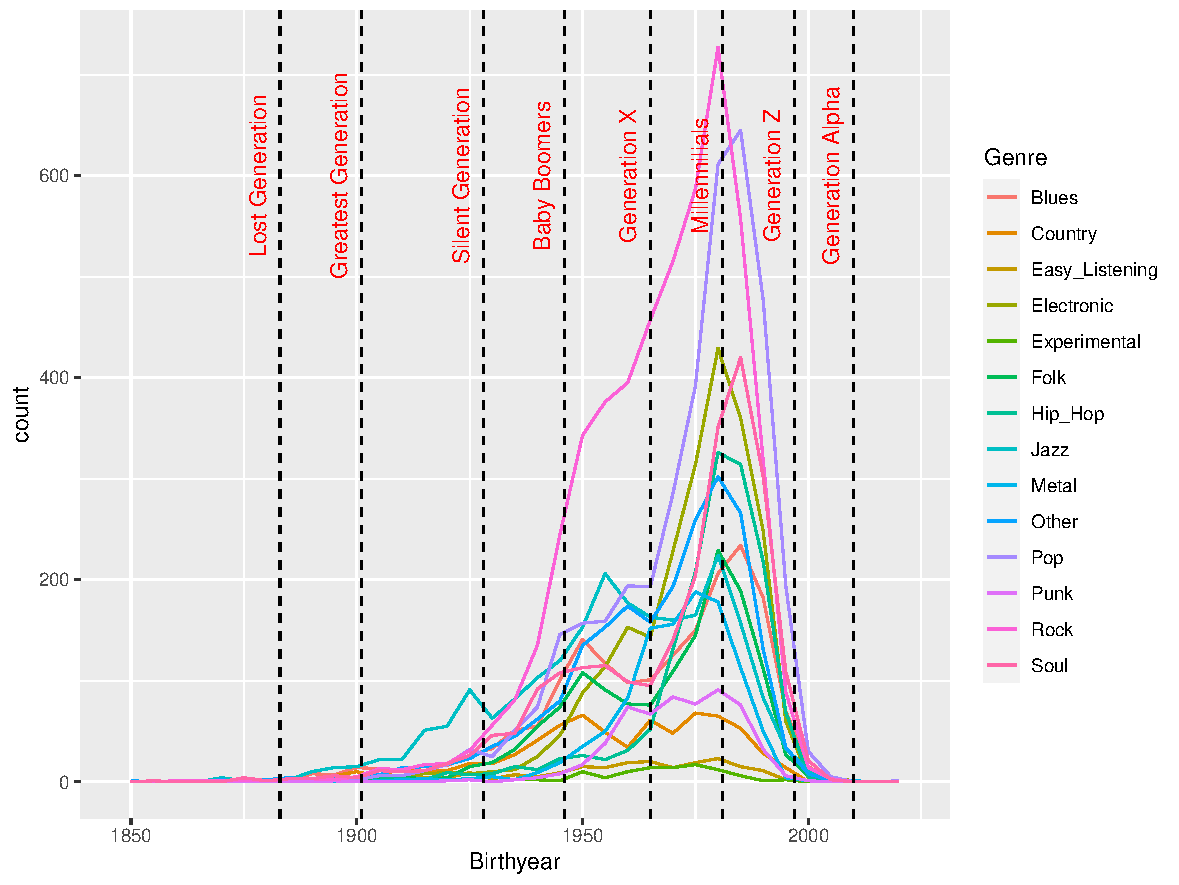
\includegraphics[width = 9cm]{first_plot.pdf}
    \caption{\textit{The change in number of musicians representative of various genres, born in 5-year cohorts since 1850.}}
    \label{fig:linegraph_genre_over_time}
\end{figure}

\section{Discussion}
The first plot, as seen in \autoref{fig:linegraph_genre_over_time}, already shows a few trends, such as jazz and rock musicians starting to become more numerous at earlier times than the other groups. However, more specific trends are more difficult to discern in the current form of the data and plot. The fact that all of the lines trend upwards leading up to 1980 and then drop sharply suggests that there are other factors at play besides popularity of individual genres. These could be accounted for by calculating the proportions of musicians from specific genres by birth year, instead of the absolute number. 

Further limitations are as follows: our current analysis involves a grouping that creates an “other” category in the genres that covers quite a wide range of hard-to-categorise genres, which makes that data not very usable. We are considering creating more groups for these genres or simply excluding these genres from our analysis.

Year of birth does not point to the time a musician published their music than other variables might. To address this, we could make use of the activeYears keys in the dataset. Not all Wikipedia entries have this label though, so for those cases we might add a certain number of years to their birth year, to approximate the year in which they most likely became a professional musician.

Further research into the changes in popularity of music genres over time could research instrumentation, lyrics, timbre, composition, and other more specific aspects. Of these, lyrics would be the easiest to achieve, since these could be more easily found in textual databases and thus do not require any analysis of the auditory aspects of the music. Additionally, the research could be expanded to track the “lifespan” of different genres, comparing the longevity of different genres’ popularity. 

\section{Future Plan}
Wednesday Morning:
\begin{itemize}
    \item Fix up the basic genre/birthyear data to control for the amount of entries and create the final plot.
    \item Run alternate analyses to check if this changes our conclusions drastically. 
    \item Settle on conclusions for the basic question, write down results and discussion bits for the final report!!!
\end{itemize}
Wednesday Afternoon:
\begin{itemize}
    \item Explore expanding our research: 
    \begin{itemize}
        \item Can we do the song lyric thing?
        \item Add genre lifespan into the mix (should be easier than the song lyric thing).
    \end{itemize}    
    \item Collect results from expanded research, add to the final report.
\end{itemize}
Thursday Morning:
\begin{itemize}
    \item Wrap up any remaining data processing/visualisation.
    \item Make a final report draft, work out the narrative we want to follow. 
\end{itemize}    
Thursday Afternoon:
\begin{itemize}
    \item Make and practise the presentation.
\end{itemize}    
    
\printbibliography


\end{document}
